
\begin{blocksection}
\question
Consider the C code here, and assume the malloc call succeeds. Rank the value of each variable (which may be an address!) from 1 to 5 (with 1 being the least) right before bar returns.  Use the memory layout from class;  Treat all addresses as unsigned numbers. 

\begin{verbatim}
#include <stdlib.h> 

int FIVE = 5;

int bar(int x) {
    return x * x;
}

int main(int argc, char *argv[]) { 	
    int *foo = malloc(sizeof(int)); 	
    if (foo) free(foo); 	
    bar(10); //  snapshot just before it returns 	
    return 0; 
}
FIVE: _____
foo: _____
&FIVE: _____
&foo: _____
&x: _____


Memory Diagram from class for reference:
\end{verbatim}
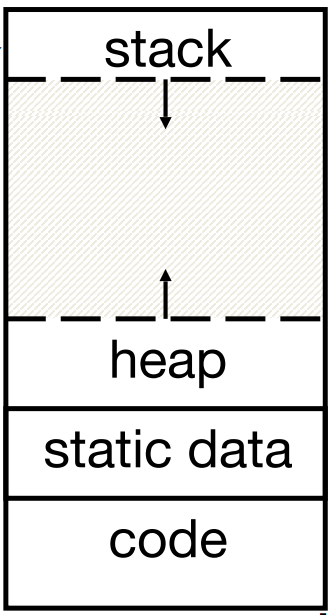
\includegraphics[scale = 0.35]{topics/c/memorydiagram.png}
0x00000000
\end{blocksection}
\begin{blocksection}
\begin{solution}
In order from lowest to highest address: \lstinline$FIVE, &FIVE, foo, &x, &foo$
\begin{verbatim}
FIVE: 1
foo: 3
&FIVE: 2
&foo: 5
&x: 4
\end{verbatim}


\lstinline$FIVE$ itself contains the value “5”, \lstinline$&FIVE$ contains the address of \lstinline$FIVE$ and since it is a global variable, it is stored statically, which means that it will be stored in the data segment. Since \lstinline$foo$ is a pointer, it contains the address of whatever it was assigned to, which in this case, is \lstinline$malloc(sizeof(int))$. As a result, \lstinline$foo$ is stored on the heap, which is above the data segment. \lstinline$&foo$ itself lives on the stack, since the space to store the pointer to the data that foo holds is allocated on the stack. This is above the heap. \lstinline$x$ is a local variable, so it also gets allocated on the stack; the reason \lstinline$&x$ is smaller than \lstinline$&foo$ is simply because the stack grows downwards, and during the execution of the program, the space for \lstinline$foo$ is allocated before the space for \lstinline$x$.
\end{solution}

\end{blocksection}